\chapter{Why Do You Want to Be an Entrepreneur?}

This chapter follows Session 6, Part 1 of MIT OpenCourseWare's Nuts and Bolts of New Ventures, curated for these notes by LazyingArt LLC through Video2Book. The lecture is Bob Jones's answer to a question Joseph Hadzima had placed near the beginning of the course: beyond the mechanics of incorporation, customers, projections, and funding, what does it mean for a person to choose entrepreneurship? The mathematical content is deliberately light, but not absent. The central formula is Hadzima's expectation heuristic, and the rest of the lecture uses statistics, update rules, and back-of-the-envelope checks to discipline a subject that is otherwise easily swallowed by mythology.

\section{From Venture Mechanics to Founder Fit}

The session begins as a course-level handoff. Hadzima reminds us that the preceding meetings have dealt mostly with factual and operational questions: whether a venture needs a corporation, how a founder finds customers, how one thinks about projections, negotiation, and finance. But there was also a more personal question at the start: is this right for us?

Jones does not immediately answer that question. He first asks the room to evaluate the course itself. That opening exchange matters because it models the same principle the course has been teaching. A practical entrepreneurship course should practice customer discovery on itself. The students answer in the language of utility: the course distilled a large process into six sessions, gave non-business people a usable structure, and made practical topics such as negotiation, numbers, pitching, and financing less mysterious.

The opening therefore does two things at once. It closes the loop on the prior nuts-and-bolts material, and it creates permission to leave pure technique behind. Jones's agenda is stories, the hard parts that rarely get discussed, lessons, and then a wrap-up. We should not treat this as an inspirational appendix. It is the founder-fit chapter of the course.

\section{Myths, Facts, and the Expectation Reset}

Jones first names the mythology. There is a popular story in which money is abundant, the brilliant idea attracts investors almost automatically, and a boot camp can hand us a magic formula for success. The course could have amplified that story. Instead, Jones frames the choice as a moral one: sell the myths, or tell the facts.

The lecture's first compact equation appears here, credited on the slide to Hadzima.

\begin{figure}
\centering

\includegraphics[width=0.95\linewidth]{lecture_09_figure_02.png}
\caption{Hadzima's expectation heuristic as shown in the lecture.}
\end{figure}

The slide gives the formula in slash form. The clean note form is
\begin{equation}
H=\frac{R}{E}.
\end{equation}
The transcript supplies the meanings of the letters:
\begin{equation}
\text{happiness}
=
\frac{\text{reality}}{\text{expectations}}.
\end{equation}
This is not a law of psychology and it is not a derivation. It is a heuristic for expectation management. If expectations are inflated by hype, then the denominator is too large, and the lived result is disappointment. If expectations are calibrated to reality, the same reality can be interpreted more sanely.

One simple way to read the formula is as a sensitivity statement:
\begin{align}
H &= \frac{R}{E},\\
\text{if } R \text{ is fixed and } E \text{ rises},\quad H &\text{ falls},\\
\text{if } R \text{ is fixed and } E \text{ is made realistic},\quad H &\text{ becomes more stable}.
\end{align}
This is the reason the lecture talks about hard facts before it talks about motives. The work is not to make entrepreneurship bleak. The work is to remove false denominators.

Jones then gives the facts in rough form. Entrepreneurship is hard. Most startups fail. Investors generally assume that we are likely to fail, even if we are smart, charming, and decent people. Many founders compete for the same talent, capital, and attention. Many will not get the money.

Later in the lecture, the failure-rate claim appears as a stark slide.

\begin{figure}
\centering

\includegraphics[width=0.95\linewidth]{lecture_09_figure_05.png}
\caption{The lecture's visible failure-rate framing. The statistic is used as a lecture claim, not as a sourced universal law.}
\end{figure}

The useful note form is cautious:
\begin{equation}
\text{survival after two years}\approx 10\%.
\end{equation}
Jones also states the claim verbally in a broader form:
\begin{equation}
\text{startup failure rate}\approx 80\%\text{ to }90\%.
\end{equation}
He immediately cautions that industries use different metrics. In food, for example, one question is whether the product is still on the shelf two years later. Other industries ask different questions. So the number should not be hardened into a theorem. It is an expectation reset.

\begin{remark}
The lecture's mathematical spine is intentionally thin. The formula \(H=R/E\), the survival statistic, and the later hypothesis-testing loop are not substitutes for market evidence. They are framing devices that keep us from treating entrepreneurship as either glamour or doom.
\end{remark}

\section{The First Flop}

Jones now moves from formula to story. He tells us about springboard diving with his teenage daughter. The details are not decorative. They slow down the moment before the analogy becomes useful.

A new diver can learn the board, gain some altitude, learn a few basic moves, and then reach the first real test. Jones's daughter is sent to the high board. She is told to turn backward, tuck, fall, listen for the command, come out of the tuck, find the water, and enter head first. The second time this is not so frightening. The first time, it feels like death. She panics, misses the exit, and lands in a full back flop.

The entrepreneurial analogy follows exactly. When we try something we have not done before, the first serious failure hurts. It hurts especially if we have lived a life of high achievement and are accustomed to being rewarded for intelligence and work ethic. Then comes the fork:
\begin{equation}
\text{painful flop}
\longrightarrow
\begin{cases}
\text{stop},\\
\text{try again}.
\end{cases}
\end{equation}
Jones is careful not to romanticize the second branch. For many people, stopping is the right decision. Entrepreneurship is not a moral test that everyone must pass. But a few people, in his joking phrase, have a different wiring. They say: that did not kill me; I am going to do it again.

\subsection{Question \& Answer}

Question: After the first hard failure, why would anyone continue?

Answer: Not because failure is pleasant, and not because persistence is always wise. The lecture's answer is narrower. Some people discover that the first flop is survivable. If it is survivable, it can become information. The diver goes back up the ladder not because the pain was imaginary, but because the pain did not settle the question. Likewise, the founder who continues does not deny the failure. The founder refuses to treat one failure as the final measurement of the person.

This is the first conceptual obstacle in the lecture. If failure is read as identity, the story ends. If failure is read as experience, the next question becomes: what did we learn?

\section{Failure, Rejection, and the Social Cost of Starting Up}

The lecture next accumulates cases. Trevor starts young, appears successful, and then loses the visible symbols of success: car, relationship, independence, status. The lesson is not that humiliation is noble. It is that failure was not fatal. Trevor later becomes successful, but only after living with the taste of failure and becoming what Jones calls a perpetual learner.

Jones draws the first explicit trait conclusion:
\begin{equation}
\text{entrepreneurial survival}
\not\equiv
\text{intelligence}
\quad\text{and}\quad
\text{entrepreneurial survival}
\not\equiv
\text{creativity}.
\end{equation}
The trait he emphasizes is adaptability:
\begin{equation}
\text{key trait} \approx \text{adaptability}.
\end{equation}

Laura's story adds customer validation. She leaves a senior corporate role, assumes she is the smartest person in the room, is quickly shaken by hard questions, and goes through more than one wrong idea. Her second business consumes substantial personal money before she recognizes that the prospects are not going to use the product. The compressed lesson is one the course has been repeating:
\begin{equation}
\text{validate}
\longrightarrow
\text{talk to customers}
\longrightarrow
\text{learn whether they want it}.
\end{equation}
If customers do not want it, we cannot sell it by force of enthusiasm.

Laura's later success comes through reach. She asks for help from a real-estate executive without initially realizing the scale of his network. When he says he wants the product for all his agents, the scale changes:
\begin{equation}
\text{one useful conversation}
\longrightarrow
11{,}000\ \text{possible users}.
\end{equation}
Again, this is not a formula for distribution. It is an example of why talking to people can reveal a market path that private reasoning does not.

Jones then turns to loneliness. He uses a Jack-and-Jill parable, though parts of the transcript are garbled, to make a clear point: uncertainty that is ordinary inside a startup may sound terrifying at home. If a founder says, ``I do not know what I am doing,'' the spouse may hear existential danger: mortgage, children, savings, risk. The founder then learns to hide self-doubt at work or at home. That creates isolation.

The rejection is not occasional. Potential clients say no. Partners say no. Investors say no. Potential employees take safer jobs. A founder who has been rewarded for competence may suddenly live in a world where competence is not enough to prevent repeated refusal. Jones then adds a harsher example: investors can be the wrong people, and intellectual property can be poorly protected. His sidebar is direct:
\begin{itemize}
\item Do not raise money from the wrong people.
\item Protect intellectual property, especially a secret algorithm, formula, or defensible business method.
\end{itemize}

The emotional companions of this phase are anxiety, self-doubt, and imposter syndrome. The founder has been presenting as the capable captain of the ship while privately wondering whether that is true. That is the setup for the next turn in the lecture.

\section{Failure as Evidence, Not Identity}

The question Jones asks is simple: is there hope for us? His first answer is community. Ordinary friends may not understand why the founder is not simply working in a stable job. The founder's choices can look irrational from the outside. So he recommends finding a community of people who are similarly wired, people for whom uncertainty, ambition, and repeated attempts are intelligible.

Then he shifts gears. The word ``pivot'' can sound like a polite synonym for not knowing what one is doing. Jones accepts that, but reframes it using scientific method. A scientist articulates a hypothesis and tests it. If the hypothesis fails, the next step is not shame. The next step is another hypothesis.

The lecture's cleanest update rule is therefore
\begin{equation}
\text{hypothesis}
\longrightarrow
\text{test}
\longrightarrow
\text{evidence}
\longrightarrow
\text{revised hypothesis}.
\end{equation}

\begin{figure}
\centering
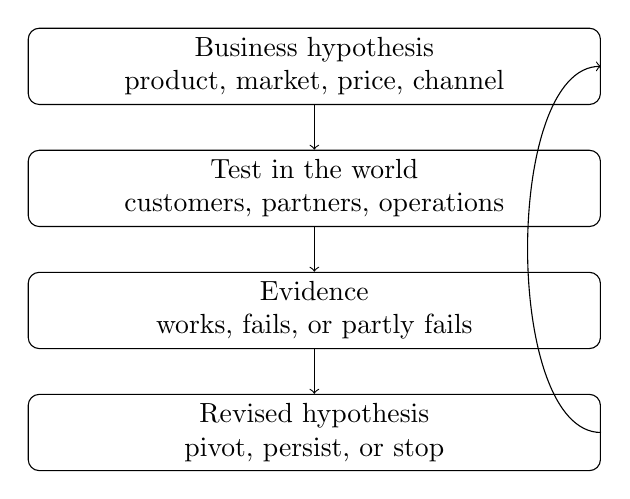
\begin{tikzpicture}[x=1cm,y=1cm]
\node[draw, rounded corners, align=center, text width=0.58\linewidth] (h) at (0,0) {Business hypothesis\\product, market, price, channel};
\node[draw, rounded corners, align=center, text width=0.58\linewidth] (t) at (0,-1.55) {Test in the world\\customers, partners, operations};
\node[draw, rounded corners, align=center, text width=0.58\linewidth] (e) at (0,-3.10) {Evidence\\works, fails, or partly fails};
\node[draw, rounded corners, align=center, text width=0.58\linewidth] (r) at (0,-4.65) {Revised hypothesis\\pivot, persist, or stop};
\draw[->] (h) -- (t);
\draw[->] (t) -- (e);
\draw[->] (e) -- (r);
\draw[->] (r.east) .. controls (2.4,-4.65) and (2.4,0) .. (h.east);
\end{tikzpicture}
\caption{A transcript-backed reconstruction of Jones's hypothesis-testing loop. This is not copied from a slide; it is a compact rendering of the spoken method.}
\end{figure}

We can write the update more explicitly. Let \(B_n\) denote the current business hypothesis at attempt \(n\), and let \(D_n\) denote the evidence produced by testing it. Then the practical update is
\begin{equation}
B_{n+1}=\operatorname{revise}(B_n,D_n).
\end{equation}
This is not meant as a formal algorithm. It is a discipline of interpretation. The point is that a failed business path is not automatically the same thing as a failed founder:
\begin{equation}
\text{failed hypothesis}\neq\text{failed person}.
\end{equation}

\subsection{Question \& Answer}

Question: If most startups fail, how should we think about failure?

Answer: We should not make it smaller than it is. Failure can cost money, time, status, and relationships. But in the lecture's scientific framing, failure is also evidence. It tells us that one hypothesis, one market, one execution path, or one timing assumption did not work. The productive response is not denial. The productive response is revision.

This is why Jones's horse analogy works. We may be a good jockey on the wrong horse. The answer is not to insist that the horse is fine. The answer is to find a better horse.

\section{Supports: Community, Advisors, and Self-Management}

The hypothesis loop is not something a founder should try to run alone. Jones recommends a business advisory board, and he sharply distinguishes it from a board of directors.

A board of directors represents shareholders. It has fiduciary duties. It can be empowered, and sometimes obligated, to remove the founder. That is not always the right room in which to say, ``I have no idea what to do next.''

A business advisory board is different. It has no fiduciary control over the company. It is a place to collect people who know things we do not know, who want the venture to succeed, and who can help in narrow but crucial domains. Jones's beverage example makes the point concretely. He and a scientist friend had a small drink product and needed manufacturing help at quantities below an unaffordable large-bottle threshold:
\begin{equation}
\text{needed production scale}<2{,}000{,}000\ \text{bottles}.
\end{equation}
An advisor solved the problem quickly because the advisor knew that narrow arena.

The equity example is also instructive. Jones first thought about giving each advisor one point:
\begin{equation}
\text{proposed advisor equity}=1\%.
\end{equation}
The advisors told him that was too much and recommended half a point:
\begin{equation}
\text{revised advisor equity}=0.5\%.
\end{equation}
The point is not that every advisor should receive \(0.5\%\). The point is that sophisticated advisors can improve not only operations, but also the way the cap table is read by future investors.

Jones also emphasizes composition. We need some advisors who encourage us after we fall down. But we also need one or two who can tell us ten sensible reasons why our plan may not work. If seven are already covered and three are new, those three are precious.

Then the lecture turns from external support to bodily support. Many founders think the business must consume every hour. Jones argues that this is a bad model because founders need judgment, and judgment decays under exhaustion. The fixed constraint is
\begin{equation}
W=168\ \text{hours/week}.
\end{equation}
No founder gets more. Spending all of \(W\) on the company is not proof of seriousness. It is a path toward impaired decisions.

Jones gives a sleep comparison from literature he encountered while working in the sleep business:
\begin{equation}
5\ \text{hours/night of sleep}
\sim
\text{cognitive impairment of three drinks}.
\end{equation}
We should keep the comparison in exactly that spirit: a lecture claim used to make the decision-quality point vivid. Frayed-out entrepreneurs make bad decisions. The business may not die instantly, but it becomes more likely to die from the founder's degraded judgment.

The recommendations are plain: eat decently, exercise, walk, sleep, take care of loved ones, and do things that recharge the battery. Jones's Halloween story supplies the moral weight. Family members may remember our absence long after we forget the business emergency that caused it.

\section{Why Do It Anyway?}

At this point the lecture has made entrepreneurship look hard enough that the natural question returns: why would anybody do this?

Jones answers with several motives and does not reduce them to one. Some people feel they have to create something better. Some want to be their own boss badly enough to accept a pay cut. Some discover that corporate life simply does not fit. Some want to improve quality of life for others.

The philanthropic stories make this concrete. One entrepreneur in health-care software initially seems to be building toward investor appeal and acquisition. But when he talks about an orphanage in Venezuela, he becomes animated in a different way. Jones helps him see that the real objective may not be to build a company for acquisition as quickly as possible. It may be to build a durable company that lets him support work he deeply cares about.

Another entrepreneur brings internet access to rural Nebraska. The business does not sound glamorous until he describes a mother who has been taking her children to a library parking lot so they can use Wi-Fi for homework. When internet access reaches her home, she can cook dinner with her children for the first time in years and return to normal work hours. That is not startup mythology. It is a concrete improvement in life.

So the motive set is broad:
\begin{align}
\text{entrepreneurial motive}
\in
\{&
\text{autonomy},
\text{misfit with corporate life},
\text{service},\\
&
\text{wealth creation},
\text{love of building},
\text{technology buzz},
\text{creative discipline}
\}.
\end{align}
Jones also compares entrepreneurship with music. Creativity is not enough. We need scales, modes, time signatures, and framework. Then we need creative life inside that discipline. A good venture has the same double structure:
\begin{equation}
\text{good entrepreneurship}
\approx
\text{creativity}+\text{discipline}.
\end{equation}

\section{Practical Timing and Runway}

The final audience questions bring the lecture back to practical judgment. If it may take several attempts to build something valuable, how do we create enough runway?

Jones gives two answers. First, failed entrepreneurship does not necessarily make a person unemployable. Some companies want change agents, people who are not afraid of a blank sheet of paper and can bring creative thinking to an established organization. Second, a founder can weave in and out: work in a normal job for a while, learn, earn, calm the family situation, and later start again.

The next question is whether to build on the side while keeping a day job, or to go all in immediately. Jones argues against going all in before doing at least some market arithmetic. He refers back to the earlier session's back-of-the-envelope analysis:
\begin{align}
I_{\text{needed}}&=\text{income the venture must produce},\\
V_{\text{customer}}&=\text{economic value of one customer},\\
N_{\text{required}}&\approx \frac{I_{\text{needed}}}{V_{\text{customer}}}.
\end{align}
The final question is not just whether \(N_{\text{required}}\) can be written down. The question is whether the market can plausibly supply that many customers:
\begin{equation}
N_{\text{reachable}}\geq N_{\text{required}}.
\end{equation}
If we have not done that kind of check, Jones says it is not the right time. If we have done it, it might be the right time. The practical recommendation is small-step validation:
\begin{equation}
\text{side test}
\longrightarrow
\text{mistakes while still paid}
\longrightarrow
\text{validated pitch}
\longrightarrow
\text{full-time commitment}.
\end{equation}
This is also where passion must be disciplined. Passion is good if it gets us back up after being knocked down. Too much passion blinds us to obvious problems. In pitching and in life decisions, Jones's rule is to deploy passion wisely.

\section{Summary}

This lecture is the personal counterpart to the rest of Nuts and Bolts. The earlier sessions teach the venture mechanics; this session asks whether we can live with the human consequences of those mechanics.

The first tool is Hadzima's heuristic:
\[
H=\frac{R}{E}.
\]
The chapter is largely about reducing false expectations. The facts are difficult: most startups fail, many investors expect failure, and founders face rejection from customers, partners, investors, and employees. But failure is not only pain. In the lecture's most useful formal move, failure becomes evidence in a hypothesis-testing loop:
\[
\text{hypothesis}
\rightarrow
\text{test}
\rightarrow
\text{evidence}
\rightarrow
\text{revised hypothesis}.
\]
To survive that loop, founders need community, advisors, health, sleep, family, and a motive strong enough to survive contact with reality. Entrepreneurship has rewards for some people, but it is not for everyone. That is not a warning tacked onto the end of the course. It is one of the course's central facts.